\chapter{Ransomeware}\label{Ransomeware}

In this chapter we talk about the theoretical background of ransomeware.
In section \ref{Definition} we see the needed terminology to have a full understanding of the project.
Next we dig deeper in ransomeware and look at the main components of the malware. In the last section we study the evolution of ransomeware throughout the years.


\section{Definition}\label{Definition}

In this section we talk about the basic definitions to get a full understanding of the project
\subsection{Malware}

Malware is the short term for `malicious software', which refers to the software programs, who are designed to damage or do other unwanted actions on a computer system \cite{malware}. We have all kinds of malware for example: viruses, worms, trojan horses, and spyware. For this project we are focussing on another type of malware namely, ransomeware.

\subsection{Ransomeware}

Ransomeware is a type of malware, which hijacks the files on the infected computer by encryption all the files. The only way the ransomeware will decrypt the files, is when the victim pays the asked ransom money. The strength of the encryption and asked ransom money vary, but as we will see in the next section, every ransomeware has the same general pattern. They only differ in the tweaks they apply in those main components. What exactly these tweaks in those main components are, how they differ from each other and how they evolve over time, we will see in section \ref{History of Generations}, where we take a closer look at the different generations of ransomeware.


\section{Workflow}\label{workflow}

In this section we take a closer look at the workflow of the ransomeware. In every type of ransomeware we find the same workflow. Every ransomware starts with the search for a victim. After finding a victim it has to look for a weak spot, what makes it possible to install the ransomeware. When the weak spot is found, the ransomware install itself and hijacks the files of the victim by encryption. After the completion of the installation the ransomeware notifies the victim and asks for ransom money. Only when the ransom is paid, the ransomeware will decrypt the files of the victim.

In the next subsections we talk about each step of the workflow in greater detail.

\subsection{The search for a victim}\label{search}

The first step you need to do, when a criminal wants to use ransomeware is finding a victim. Nowadays with the internet is this very. A criminal can get in touch in a variatie of ways.

\subsubsection{E-mail}

The popular way is by email. Most of the time criminals craft an email with social engineering techniques, which causes the victim to open the attachment in the email. This attachments seems harmless for the victim but is in reality the ransomeware, which immediately infects the victim's computer when opened.


\begin{figure}[H]
    \centering 
    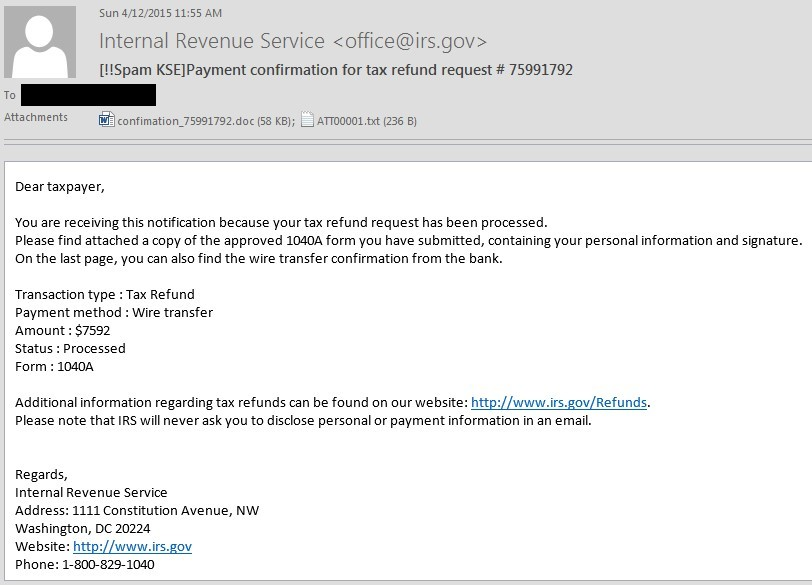
\includegraphics[height=7cm]{example_ransomemail}
    % \caption{An example of a specially crafted email by a criminal, which causes the reader to open the attachment.
    \caption[]{An example of a specially crafted email by a criminal, which causes the reader to open the attachment.\protect\footnotemark}
    \label{ransomemail}
\end{figure}
\footnotetext{Source: http://i1-news.softpedia-static.com/images/news2/Users-in-the-US-Targeted-with-Ransomware-Via-Tax-Return-Flavored-Emails-478465-2.jpg}

\subsubsection{Removable Device}

Another methode is a removable device. This can be a USB-stick, CD or even a mobile phone. The device can be plugged in by the criminal himself and he let lying around intentionally some removable devices in the hope the finder would connect it with the computer.

In the next section we talk step namely finding a way to trick the victim.

\subsection{Tricking the victim}

As we said in in \ref{search} can way reach a victim in a variatie of ways. But reaching the victim is not enough. The ransomeware has still to execute.

If we reach for example of the email in \ref{search}. The user cannot have any clue that the attachment is malicious and the ransomeware needs still to execute when opened. A possible trick is \textbf{the Right to left notation}.
\subsubsection{Right to left notation}

the Right to left notation is a trick which makes use of a special character, what causes everything behind it to inverse.

\subsection{Compromising the victim's machine}\label{Compromising}

Encryption
\subsection{Notifying the victim}\label{notify}


\subsection{decryption}\label{decryption}



\section{History of Generations}\label{History of Generations}